\chapter{Revisão Estruturada da Literatura}
\label{cap:revisao_sistematica}

Este capítulo documenta o planejamento e a condução da revisão estruturada dos estudos primários que compõem a base científica desta monografia, elaborados em conformidade com as diretrizes de \citeonline{kitchenham2007} para revisões estruturadas na Engenharia de Software. Para a identificação dos estudos primários, adotou-se a base de dados Scopus como motor central de busca automatizada, visto que seu acervo indexa de maneira integrada as publicações das principais bibliotecas digitais de Ciência da Computação e Segurança Cibernética.

\section{Protocolo da Revisão}
\label{sec:rsl_protocolo}

O protocolo desta revisão estruturada da literatura baseia-se no modelo formal de revisão sistemática de \citeonline{kitchenham2007} para reduzir o viés de seleção e favorecer a auditabilidade e a replicabilidade do estudo.


\subsection{PICO e String de Busca}
\label{subsec:rsl_string_busca}

Para estruturar a estratégia de busca, adotou-se a abordagem baseada nos critérios PICO e PICOC recomendados por \citeonline{pai2004} e \citeonline{kitchenham2007}. Originalmente proposto na medicina baseada em evidências, o acrônimo PICO organiza a questão de pesquisa em quatro elementos: população estudada, intervenção aplicada, comparação de controle e resultado mensurado, representados como um diagrama de Venn na Figura~\ref{fig:rsl_pico} \cite{pai2004}.

\begin{figure}[!htbp]
    \centering
    \caption{Representação Visual do Protocolo PICO.}
    \label{fig:rsl_pico}
    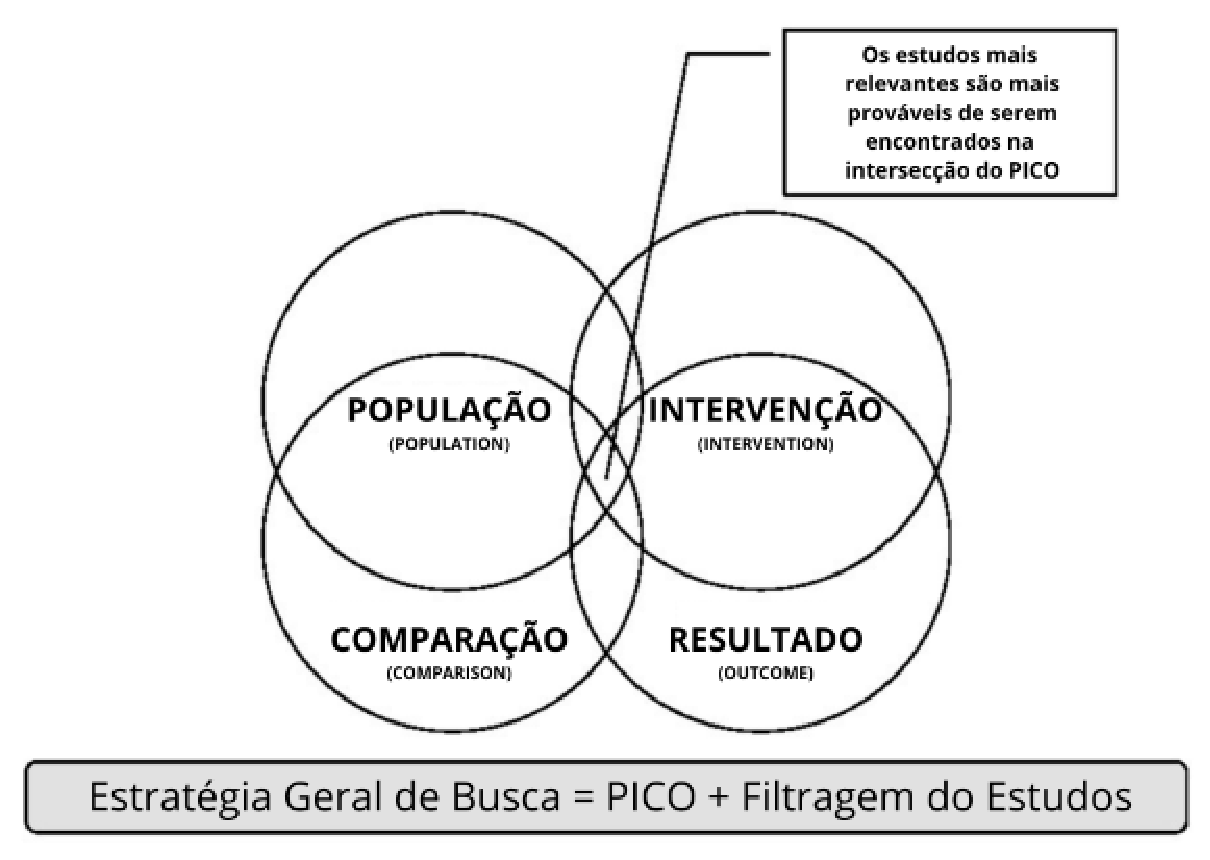
\includegraphics[width=0.68\textwidth]{figuras/pico.eps}
    \fonte{Adaptado de \citeonline{pai2004}.}
\end{figure}
\FloatBarrier

Na Engenharia de Software, \citeonline{kitchenham2007} estendem esse modelo para o formato PICOC ao incluir a faceta de Contexto. Neste trabalho, o protocolo foi adaptado para a estrutura \textbf{PIO}: a faceta de Comparação foi omitida por inexistir grupo de controle único na busca exploratória, enquanto o Contexto, referente a sistemas distribuídos, microsserviços e nuvem, foi incorporado à População para evitar restrição booleana excessiva. Assim, a População abrange sistemas de software e infraestruturas distribuídas em nuvem, a Intervenção reúne mecanismos de monitoramento e gestão de \textit{logs} de segurança em tempo de execução e os Resultados compreendem conformidade regulatória e maturidade cibernética, conforme a Tabela~\ref{tab:rsl_protocolo_pio}.

\begin{table}[!htbp]
    \centering
    \caption{PICO adaptado (estrutura PIO).}
    \label{tab:rsl_protocolo_pio}
    \small
    \begin{tabular}{p{2.4cm}p{3.4cm}p{8.7cm}}
        \hline
        \textbf{Elemento} & \textbf{Termo Central} & \textbf{Sinônimos e Termos Relacionados} \\ \hline
        \textbf{População (P)} & \textit{Software systems and digital infrastructure} & ``software system*'', ``software application*'', ``cloud infrastructure'', ``cloud platform*'', ``microservice*'', ``containerized environment*'', ``distributed system*'', ``web application*'', ``information system*'', ``IT infrastructure'' \\ \hline
        \textbf{Intervenção (I)} & \textit{Security log management} & ``log management'', ``audit log*'', ``audit logging'', ``security monitoring'', ``runtime security monitoring'', ``security telemetry'', ``SIEM'', ``security information and event management'', ``XDR'', ``HIDS'', ``host-based intrusion detection'', ``intrusion detection system'', ``intrusion detection'', ``security audit'', ``Wazuh'', ``event correlation'', ``threat detection'', ``security operation center'', ``SOC'', ``incident response'', ``MITRE ATT\&CK'' \\ \hline
        \textbf{Resultados (O)} & \textit{Regulatory compliance} & ``regulatory compliance'', ``security compliance'', ``compliance evaluation'', ``CIS Control*'', ``security maturity'', ``security maturity model'', ``security posture'', ``security governance'', ``audit compliance'', ``security assessment'', ``NIST'', ``security framework*'', ``compliance framework*'' \\ \hline
    \end{tabular}
    \fonte{Elaborado pelo autor.}
\end{table}
\FloatBarrier

A \textit{string} foi construída com o operador lógico \texttt{OR} entre os sinônimos de cada elemento e o operador \texttt{AND} para conectar as três facetas, aplicando a diretiva \texttt{TITLE-ABS-KEY} na base Scopus:

\begin{quote}
\footnotesize
\sloppy
\texttt{TITLE-ABS-KEY ( ( "software system*" OR "software application*" OR "cloud infrastructure" OR "cloud platform*" OR "microservice*" OR "containerized environment*" OR "distributed system*" OR "web application*" OR "information system*" OR "IT infrastructure" ) AND ( "log management" OR "audit log*" OR "audit logging" OR "security monitoring" OR "runtime security monitoring" OR "security telemetry" OR "SIEM" OR "security information and event management" OR "XDR" OR "HIDS" OR "host-based intrusion detection" OR "intrusion detection system" OR "intrusion detection" OR "security audit" OR "Wazuh" OR "event correlation" OR "threat detection" OR "security operation center" OR "SOC" OR "incident response" OR "MITRE ATT\&CK" ) AND ( "regulatory compliance" OR "security compliance" OR "compliance evaluation" OR "CIS Control*" OR "security maturity" OR "security maturity model" OR "security posture" OR "security governance" OR "audit compliance" OR "security assessment" OR "NIST" OR "security framework*" OR "compliance framework*" ) )}
\end{quote}

\FloatBarrier

\subsection{Questões Secundárias de Pesquisa}
\label{subsec:rsl_questoes_secundarias}

As doze questões secundárias derivam da Questão Principal de Pesquisa da Seção~\ref{subsec:intro_gqm} a partir das facetas do protocolo PIO e abrangem validação empírica, desafios operacionais e lacunas da literatura, conforme a Tabela~\ref{tab:rsl_questoes_secundarias}.

\begin{table}[!htbp]
    \centering
    \caption{Questões secundárias de pesquisa.}
    \label{tab:rsl_questoes_secundarias}
    \small
    \begin{tabular}{p{1.2cm}p{13.2cm}}
        \hline
        \textbf{Nº} & \textbf{Questão Secundária de Pesquisa} \\ \hline
        1 & Quais tipos de arquiteturas de software e ambientes de infraestrutura são investigados nas soluções de monitoramento de segurança em \textit{runtime}? \\ \hline
        2 & Quais domínios de aplicação ou setores são abordados nos estudos primários? \\ \hline
        3 & Quais tecnologias e plataformas de telemetria de segurança em \textit{runtime} são propostas ou avaliadas? \\ \hline
        4 & Como é realizada a coleta, centralização, decodificação e preservação dos \textit{logs} de auditoria nos estudos? \\ \hline
        5 & Quais ferramentas específicas, de código aberto ou proprietárias, são empregadas nas soluções implementadas? \\ \hline
        6 & Quais normas e \textit{frameworks} de cibersegurança são utilizados como referência de conformidade nos estudos? \\ \hline
        7 & De que maneira o CIS Control 8 ou controles equivalentes são abordados, implementados ou avaliados? \\ \hline
        8 & Quais métricas, escalas graduais ou modelos de avaliação de maturidade são aplicados para quantificar o grau de conformidade ou segurança alcançado? \\ \hline
        9 & O estudo realiza diagnóstico do estado de conformidade antes da intervenção e como esse estado inicial é estabelecido e documentado? \\ \hline
        10 & Qual método de pesquisa empírica foi utilizado para validar a solução proposta? \\ \hline
        11 & Quais são as principais limitações e desafios operacionais relatados na implementação de telemetria de segurança em \textit{runtime}? \\ \hline
        12 & Quais lacunas de pesquisa e direções futuras são apontadas pelos autores no campo de conformidade regulatória e monitoramento contínuo? \\ \hline
    \end{tabular}
    \fonte{Elaborado pelo autor.}
\end{table}
\FloatBarrier

\subsection{Critérios de Inclusão e Exclusão}
\label{subsec:rsl_criterios}

Foram estabelecidos critérios de inclusão e de exclusão para selecionar os estudos primários que fornecem evidências diretas às questões secundárias de pesquisa \cite{kitchenham2007}, dispostos nas Tabelas~\ref{tab:rsl_criterios_inclusao} e~\ref{tab:rsl_criterios_exclusao}.

\begin{table}[!htbp]
    \centering
    \caption{Critérios de inclusão da revisão estruturada da literatura.}
    \label{tab:rsl_criterios_inclusao}
    \small
    \begin{tabular}{p{1.2cm}p{13.2cm}}
        \hline
        \textbf{Nº} & \textbf{Critério de Inclusão} \\ \hline
        1 & O estudo propõe, implementa ou avalia soluções de monitoramento de segurança em tempo de execução, gestão centralizada de \textit{logs} de auditoria ou plataformas de detecção e resposta correlatas. \\ \hline
        2 & O contexto de aplicação envolve sistemas de software distribuídos, infraestruturas em nuvem, microsserviços ou contêineres. \\ \hline
        3 & O estudo avalia conformidade regulatória, maturidade de segurança, postura cibernética ou alinhamento a normas e \textit{frameworks} de segurança da informação. \\ \hline
    \end{tabular}
    \fonte{Elaborado pelo autor.}
\end{table}

Um critério preliminar que exigia validação empírica foi arquivado por orientação acadêmica conforme \citeonline{kitchenham2007}, de modo a não descartar contribuições relevantes sem validação prévia e tratar o método de validação empírica na Seção~\ref{subsec:rsl_qs10}.

\begin{table}[!htbp]
    \centering
    \caption{Critérios de exclusão da revisão estruturada da literatura.}
    \label{tab:rsl_criterios_exclusao}
    \small
    \begin{tabular}{p{1.2cm}p{13.2cm}}
        \hline
        \textbf{Nº} & \textbf{Critério de Exclusão} \\ \hline
        1 & Publicações em idiomas diferentes de inglês ou português. \\ \hline
        2 & Publicações duplicadas, mantendo-se apenas a versão mais completa. \\ \hline
        3 & Resumos expandidos, \textit{keynotes}, tutoriais, estudos secundários ou trabalhos sem revisão por pares. \\ \hline
        4 & Estudos restritos à análise estática de código-fonte, sem contemplar monitoramento em tempo de execução. \\ \hline
        5 & Estudos de \textit{logging} voltados exclusivamente a desempenho ou depuração funcional, sem foco em segurança ou conformidade. \\ \hline
        6 & Estudos cujo foco principal seja hardware físico, dispositivos conectados, redes de telecomunicações ou aspectos jurídicos sem artefatos técnicos de engenharia de software. \\ \hline
    \end{tabular}
    \fonte{Elaborado pelo autor.}
\end{table}
\FloatBarrier

\subsection{Recorte Temporal e Idiomático}
\label{subsec:rsl_recorte}

O protocolo delimitou o recorte temporal de 2015 a 2026 e o recorte idiomático aos idiomas inglês e português. O marco inicial de 2015 reflete a consolidação das arquiteturas nativas em nuvem, dos microsserviços e da orquestração de contêineres, momento em que os desafios de observabilidade e auditoria de cargas efêmeras assumiram o formato investigado nesta pesquisa. Já a restrição aos idiomas inglês e português assegura a cobertura das principais bases internacionais de Computação e de eventuais estudos nacionais voltados ao contexto regulatório brasileiro.


\subsection{Procedimento de Triagem e Extração}
\label{subsec:rsl_procedimento}

A triagem e o gerenciamento bibliográfico foram conduzidos na plataforma \textit{Evidentia} com registro auditável das decisões segundo o PRISMA \cite{kitchenham2007}. Na primeira etapa de seleção, realizou-se a leitura de título, resumo e palavras-chave aplicando os critérios de inclusão e exclusão. Na segunda etapa, os textos completos recuperados pelo Portal de Periódicos da CAPES foram avaliados na íntegra para confirmar a elegibilidade e extrair os dados nos 17 campos da Tabela~\ref{tab:rsl_formulario}.

\begin{longtable}{p{1.5cm}p{8.0cm}p{4.1cm}}
    \caption{Formulário de extração de dados.}\label{tab:rsl_formulario}\\
    \hline
    \textbf{Campo} & \textbf{Descrição} & \textbf{Função / Dimensão} \\ \hline
    \endfirsthead
    \caption[]{Formulário de extração de dados (continuação).}\\
    \hline
    \textbf{Campo} & \textbf{Descrição} & \textbf{Função / Dimensão} \\ \hline
    \endhead
    \hline \multicolumn{3}{r}{\footnotesize Continua na próxima página} \\
    \endfoot
    \hline
    \endlastfoot
    01 & Título do artigo & Metadados \\ \hline
    02 & Autores & Metadados \\ \hline
    03 & Ano e veículo de publicação & Metadados \\ \hline
    04 & Relevância temática para o escopo da pesquisa & Organização interna da leitura \\ \hline
    05 & Ambiente de infraestrutura & Arquitetura e infraestrutura \\ \hline
    06 & Domínio de aplicação & Domínio de aplicação \\ \hline
    07 & Tecnologias de telemetria em \textit{runtime} & Telemetria em \textit{runtime} \\ \hline
    08 & \textit{Pipeline} de gestão de \textit{logs} & Gestão de \textit{logs} de auditoria \\ \hline
    09 & Ferramental empregado & Ferramentas empregadas \\ \hline
    10 & \textit{Frameworks} normativos de referência & Normas e \textit{frameworks} \\ \hline
    11 & Abordagem da gestão de \textit{logs} e auditoria & Gestão de \textit{logs} e auditoria \\ \hline
    12 & Métricas e escalas de maturidade & Métricas e maturidade \\ \hline
    13 & Diagnóstico inicial (\textit{baseline}) & Diagnóstico prévio \\ \hline
    14 & Método de validação empírica & Validação empírica e qualidade \\ \hline
    15 & Desafios e gargalos operacionais & Limitações e desafios \\ \hline
    16 & Lacunas e trabalhos futuros & Lacunas e direções futuras \\ \hline
    17 & Justificativa do método de validação & Validação empírica e qualidade \\ \hline
\end{longtable}
\fonte{Elaborado pelo autor.}
\FloatBarrier

\section{Condução da Revisão}
\label{sec:rsl_conducao}

\subsection{Fluxo de Seleção dos Estudos}
\label{subsec:rsl_fluxo_prisma}

A busca na base Scopus para o período de 2015 a 2026 reuniu registros indexados de IEEE Xplore, ACM Digital Library, Elsevier ScienceDirect e SpringerLink, consolidando 357 itens importados no \textit{Evidentia} para triagem conforme o protocolo PRISMA 2020, conforme a Figura~\ref{fig:rsl_prisma}. Na leitura de título, resumo e palavras-chave, 322 registros foram descartados pelos critérios de exclusão, com maior incidência de trabalhos fora do escopo de engenharia de software e de publicações secundárias ou sem revisão por pares. Dos 35 artigos selecionados para leitura integral, 6 não tiveram o texto completo acessível no portal da CAPES, restando 29 estudos primários incluídos na amostra.

Além dos estudos primários, foram incorporados cinco documentos oficiais brasileiros para apoiar a análise regulatória: o guia do PPSI 2.0 instituído pela Portaria SGD/MGI nº 9.511/2025 \cite{portaria9511_2025,ppsi2026}, a Instrução Normativa SGD/MGI nº 4/2026 \cite{in4_2026}, a Norma Complementar nº 21/IN01/DSIC/GSI-PR \cite{nc21_2014}, a Instrução Normativa GSI/PR nº 5/2021 \cite{ingsi5_2021} e o Acórdão nº 2.387/2024 do TCU \cite{tcu2387_2024}. As análises quantitativas e percentuais deste capítulo consideram exclusivamente os 29 estudos científicos primários.

\begin{figure}[!htbp]
    \centering
    \caption{Fluxo de seleção dos estudos (PRISMA 2020).}
    \label{fig:rsl_prisma}
    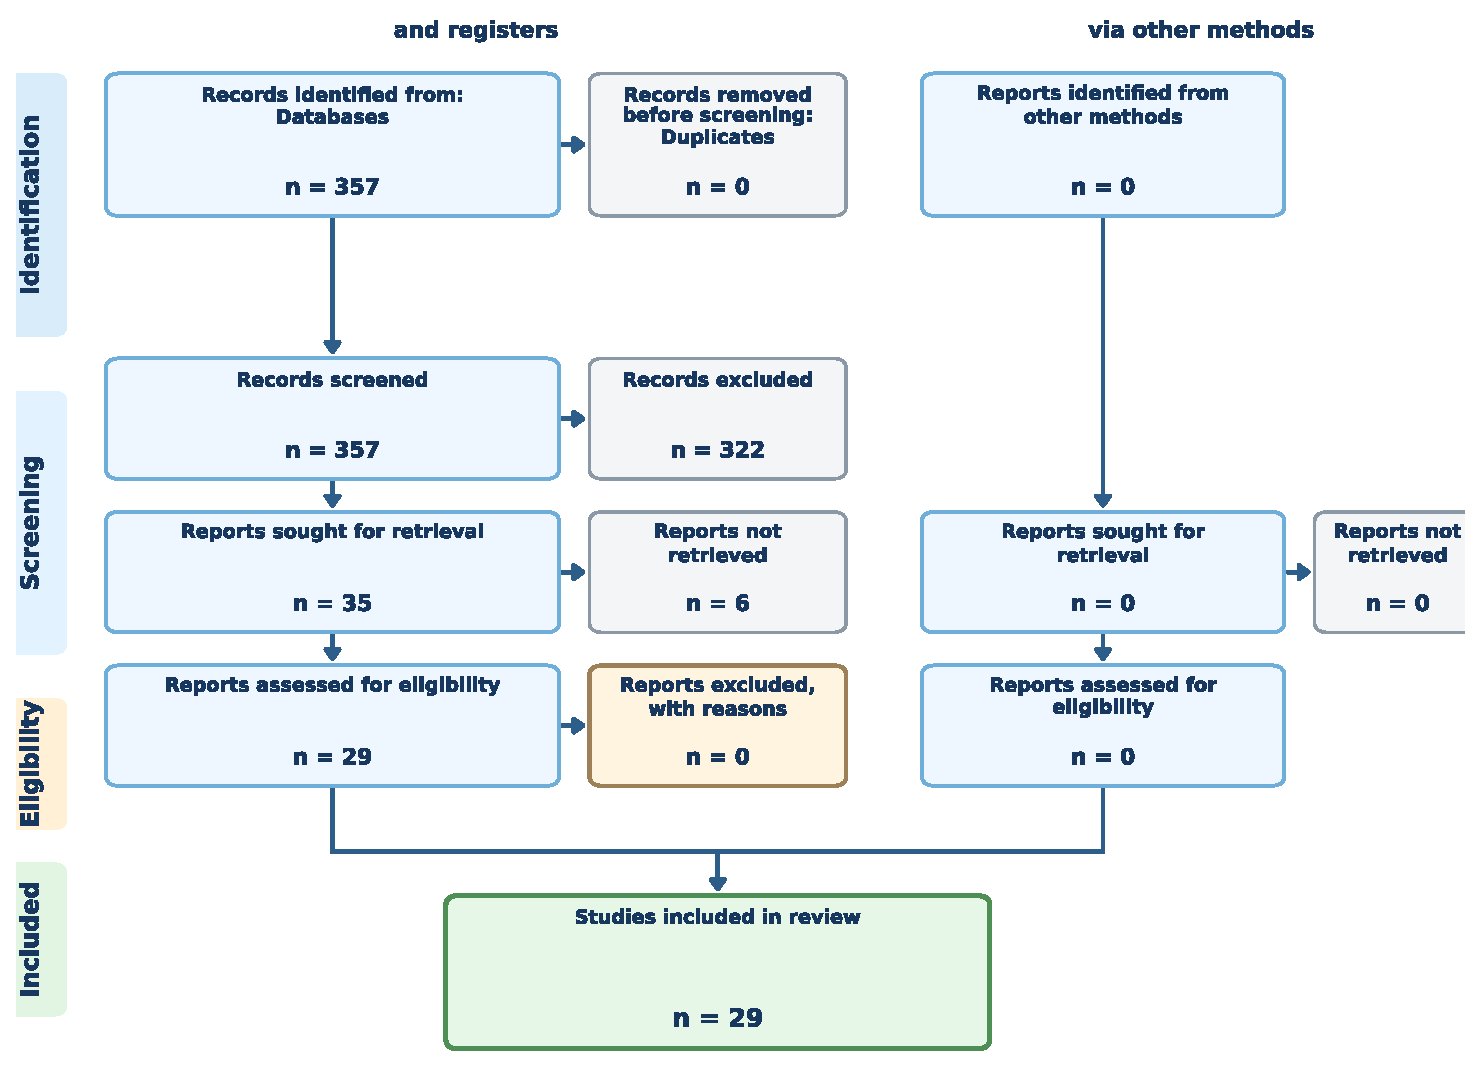
\includegraphics[width=\textwidth]{figuras/prisma.eps}
    \fonte{Elaborado pelo autor.}
\end{figure}
\FloatBarrier

\subsection{Artigos Selecionados}
\label{subsec:rsl_amostra}

{\small\setlength{\tabcolsep}{4pt}
\begin{longtable}{p{8.9cm}p{2.2cm}p{2.9cm}}
    \caption{Estudos primários selecionados.}\label{tab:rsl_amostra}\\
    \hline
    \textbf{Estudo} & \textbf{Veículo} & \textbf{Validação Empírica} \\ \hline
    \endfirsthead
    \caption[]{Estudos primários selecionados (continuação).}\\
    \hline
    \textbf{Estudo} & \textbf{Veículo} & \textbf{Validação Empírica} \\ \hline
    \endhead
    \hline \multicolumn{3}{r}{\footnotesize Continua na próxima página} \\
    \endfoot
    \hline
    \endlastfoot
SheildSentry: Linux Auditing with Gen.AI~\cite{gajra2025} & Conferência & Avaliação em pequena escala \\ \hline
Enhancing Kubernetes security with machine learning: a proactive approach to anomaly detection~\cite{darwesh2024} & Periódico & Experiment \\ \hline
Adaptive Behavioral Validation for Cloud Security Posture Management with AI-Driven Alert Prioritization~\cite{joshisabhaya2026} & Periódico & Experiment \\ \hline
Enhancing DFIR in orchestration Environments: Real-time forensic framework with eBPF for windows~\cite{jin2025} & Periódico & Experiment \\ \hline
Continuous auditing and threat detection in multi-cloud infrastructure~\cite{torkura2021} & Periódico & Experiment \\ \hline
Explainable Anomaly Detection in Cloud-Native Systems via RAG-Enhanced Vector Retrieval~\cite{devarajulu2025} & Conferência & Experiment \\ \hline
Design and Implementation of an Open-Source Security Framework for Cloud Infrastructure~\cite{shao2026a} & Conferência & Experiment \\ \hline
Threat Modeling and Cyber Risk Management for Mitigation of Attacks on Government XYZ Corporate Services Applications~\cite{sasmito2025} & Periódico & Estudo de caso \\ \hline
Secure Log Ingestion and Visualization Using Dockerized Graylog with Multiple Log Shippers~\cite{sushma2025} & Conferência & Experiment \\ \hline
SentinelJC: An Open-Source Tool for Cyber Incident Management in a Military Institution~\cite{acosta2025} & Conferência & Estudo de caso \\ \hline
Adaptive Runtime Security for Kubernetes using eBPF Telemetry and Machine Learning~\cite{joshisegireddy2026} & Conferência & Experiment \\ \hline
Cloud Security Posture Management: Automating Risk Detection, Compliance Enforcement, and Vulnerability Remediation in Cloud Infrastructure~\cite{ali2024} & Conferência & Simulação \\ \hline
Securing the Decentralized Edge: An Integrated Approach to Endpoint Security Monitoring and Threat Detection~\cite{bungei2026} & Conferência & Experiment \\ \hline
Posture Management in Zero Trust Container Framework~\cite{upadhyaya2025} & Conferência & Experiment \\ \hline
AI-Augmented Zero Trust Security Framework for Conversational AI Systems: A Behavioral Analytics Approach~\cite{aftab2026} & Conferência & Estudo de caso \\ \hline
AI-Enhanced Security: Mastering Multi-Cloud Posture Management~\cite{kumar2026} & Conferência & Experiment \\ \hline
Logging design patterns for cloud-native applications~\cite{albuquerque2024} & Conferência & Estudo sistemático da literatura \\ \hline
Enhancing Virtualization Security through System Call-based Anomaly Detection in Containers~\cite{zhang2025} & Conferência & Experiment \\ \hline
Integrated cybersecurity methodology and supporting tools for healthcare operational information systems~\cite{coutinho2023} & Periódico & Experiment \\ \hline
Integrated Log Management with WAZUH and OPNsense for Mitigating Brute Force Attacks in Cloud Infrastructure~\cite{setiawan2025} & Conferência & Experiment \\ \hline
C-Shield: A Holistic Solution for Secure End-to-End Kubernetes Multi-Cluster Management and Online Threat Mitigation using LLMs~\cite{kalafatidis2025} & Conferência & Experiment \\ \hline
IT Security and Privacy Standards in Comparison: Improving FedRAMP Authorization for Cloud Service Providers~\cite{giulio2017} & Conferência & Análise arquival \\ \hline
The Crucial Role of Observability in Enhancing Cloud Infrastructure Security in Financial Technology: A Framework for Proactive Threat Detection and Compliance~\cite{mahida2026} & Conferência & Simulação \\ \hline
SIEM-SC initial assessments: Towards a Sustainable and Compliant proposal for Security Information and Event Management~\cite{velasquez2025} & Periódico & Experiment \\ \hline
Information Systems Security Audits in Cameroon's Public Administration~\cite{enaw2018} & Conferência & Levantamento \\ \hline
Towards an Efficient Log Data Protection in Software Systems through Data Minimization and Anonymization~\cite{portillo2019} & Conferência & Experiment \\ \hline
Continuous Trust in multi-cloud Environments: An Evidence-Driven Security Assurance Method~\cite{shao2026b} & Conferência & Experiment \\ \hline
Research on Cross-Domain Attack Defense and Endogenous Security Mechanism in Power Dispatching Systems Based on Microservices~\cite{xu2025} & Conferência & Experiment \\ \hline
ACSP: An Adaptive Cloud-Native Security Platform Oriented to Cyber Resilience~\cite{hao2025} & Conferência & Experiment \\ \hline
\end{longtable}}
\fonte{Elaborado pelo autor.}
\FloatBarrier

\section{Resultados}
\label{sec:rsl_resultados}

Após a leitura integral dos 29 estudos primários, os dados foram extraídos segundo os 17 campos do formulário da Tabela~\ref{tab:rsl_formulario} e consolidados na matriz analítica da pesquisa. Seguindo as recomendações de síntese descritiva e quantitativa de \citeonline{kitchenham2007}, cada subseção a seguir responde de forma analítica e tabulada a uma das doze questões secundárias, obedecendo à ordem definida no protocolo.

\subsection{Quais tipos de arquiteturas de software e ambientes de infraestrutura são investigados nas soluções de monitoramento de segurança em \textit{runtime}?}
\label{subsec:rsl_qs01}

A literatura analisada evidencia o deslocamento do monitoramento de segurança para infraestruturas distribuídas, nativas em nuvem e de alta elasticidade. Nesse cenário, os \textit{clusters} Kubernetes e as malhas de microsserviços ocupam posição central, abrangendo desde serviços gerenciados em provedores públicos até implantações privadas de alta densidade \cite{joshisegireddy2026,aftab2026,shao2026a,shao2026b,devarajulu2025}. Como os \textit{pods} são efêmeros e compartilham o núcleo do sistema operacional hospedeiro, a telemetria precisa operar de forma contínua tanto no nível dos nós quanto na comunicação entre serviços \cite{darwesh2024,hao2025}.

De maneira complementar, propostas voltadas à governança de postura atuam sobre nuvens públicas, híbridas e \textit{multi-cloud}, monitorando recursos computacionais, armazenamento e políticas de identidade distribuídos entre diferentes provedores \cite{torkura2021,joshisabhaya2026,kumar2026}. Contêineres Docker isolados são empregados tanto para cargas descentralizadas na borda quanto para o empacotamento de plataformas SIEM e coletores de eventos \cite{sushma2025,bungei2026,zhang2025,velasquez2025}. Já os ambientes virtualizados locais e servidores dedicados permanecem relevantes em contextos com sistemas legados e requisitos estritos de isolamento, como defesa militar, saúde hospitalar e auditoria de sistemas operacionais Linux e Windows \cite{acosta2025,coutinho2023,setiawan2025,gajra2025}. A Tabela~\ref{tab:rsl_qs01} consolida a distribuição dessas categorias na amostra.

\begin{table}[!htbp]
    \centering
    \caption{Distribuição dos ambientes de infraestrutura investigados nos estudos primários.}
    \label{tab:rsl_qs01}
    \footnotesize
    \begin{tabular}{p{9.8cm}p{2.2cm}p{2.0cm}}
        \hline
        \textbf{Categoria Arquitetural} & \textbf{Frequência} & \textbf{Percentual} \\ \hline
        \textit{Clusters} Kubernetes e malhas de microsserviços & 10 & 34,5\% \\ \hline
        Infraestruturas em nuvem pública, híbrida, \textit{multi-cloud} e modelos \textit{cloud-native} & 7 & 24,1\% \\ \hline
        Contêineres Docker e cargas isoladas em nuvem ou borda & 6 & 20,7\% \\ \hline
        Infraestruturas virtualizadas locais e servidores dedicados & 6 & 20,7\% \\ \hline
        \textbf{Total da Amostra} & \textbf{29} & \textbf{100,0\%} \\ \hline
    \end{tabular}
    \fonte{Elaborado pelo autor.}
\end{table}
\FloatBarrier

\subsection{Quais domínios de aplicação ou setores são abordados nos estudos primários?}
\label{subsec:rsl_qs02}

A maior parte das pesquisas adota um recorte transversal voltado à tecnologia da informação corporativa e a serviços nativos em nuvem de propósito geral, cobrindo aplicações \textit{web} empresariais, comércio eletrônico em microsserviços, plataformas de inteligência artificial conversacional e centros de operações de segurança \cite{devarajulu2025,aftab2026,albuquerque2024,sushma2025,bungei2026}. Em contrapartida, são poucos os trabalhos aplicados diretamente ao setor público e à defesa, concentrados na gestão de riscos em aplicações governamentais na Indonésia \cite{sasmito2025}, na implantação de um centro de gerenciamento de incidentes nas Forças Armadas do Peru \cite{acosta2025} e em auditorias de segurança da informação em ministérios de Camarões \cite{enaw2018}, além de uma análise comparativa voltada à autorização de provedores de nuvem para agências federais norte-americanas \cite{giulio2017}. O restante da amostra abrange infraestruturas críticas reguladas nos setores de saúde hospitalar \cite{coutinho2023}, tecnologia financeira \cite{mahida2026} e despacho de energia elétrica \cite{xu2025}. A distribuição quantitativa por domínio encontra-se na Tabela~\ref{tab:rsl_qs02}.

\begin{table}[!htbp]
    \centering
    \caption{Domínios de aplicação e setores econômicos abordados nos estudos primários.}
    \label{tab:rsl_qs02}
    \footnotesize
    \begin{tabular}{p{9.8cm}p{2.2cm}p{2.0cm}}
        \hline
        \textbf{Domínio / Setor Principal} & \textbf{Frequência} & \textbf{Percentual} \\ \hline
        TI Corporativa e Serviços \textit{Cloud-Native} Gerais & 23 & 79,3\% \\ \hline
        Setor Público, Governo Eletrônico e Defesa & 3 & 10,3\% \\ \hline
        Infraestruturas Críticas Reguladas (Saúde, Finanças e Energia) & 3 & 10,3\% \\ \hline
        \textbf{Total da Amostra} & \textbf{29} & \textbf{100,0\%} \\ \hline
    \end{tabular}
    \fonte{Elaborado pelo autor.}
\end{table}
\FloatBarrier

\subsection{Quais tecnologias e plataformas de telemetria de segurança em \textit{runtime} são propostas ou avaliadas?}
\label{subsec:rsl_qs03}

Para obter visibilidade em tempo de execução sem comprometer a escalabilidade das cargas, os estudos articulam sensores em cinco camadas complementares, do núcleo do sistema operacional ao plano de controle em nuvem. No nível do núcleo, ganham destaque a instrumentação com \textit{Extended Berkeley Packet Filter}, ou eBPF, e o sensor Falco, que interceptam chamadas de sistema e eventos de processos sem alterar os binários das aplicações \cite{jin2025,joshisegireddy2026,kalafatidis2025,shao2026a,zhang2025}. Na camada de hospedeiro e perímetro, sobressai o SIEM Wazuh, adotado para centralização de registros, verificação de integridade de arquivos, avaliação automatizada de configuração e resposta ativa, muitas vezes integrado a sensores de rede e \textit{firewalls} \cite{acosta2025,bungei2026,setiawan2025,sasmito2025}. Essa cobertura amplia-se com observabilidade distribuída em malhas de serviços e trilhas administrativas de provedores em nuvem e do Kubernetes \cite{aftab2026,devarajulu2025,torkura2021,kumar2026}. A Tabela~\ref{tab:rsl_qs03} detalha as tecnologias e plataformas identificadas por camada.

\begin{table}[!htbp]
    \centering
    \caption{Categorias de tecnologias de telemetria em \textit{runtime} identificadas na amostra.}
    \label{tab:rsl_qs03}
    \footnotesize
    \begin{tabular}{p{4.8cm}p{9.2cm}}
        \hline
        \textbf{Camada de Telemetria} & \textbf{Mecanismos Técnicos Principais} \\ \hline
        Instrumentação de \textit{Kernel} via eBPF & \textit{Kprobes}, \textit{tracepoints}, Cilium, Tetragon e \textit{eBPF-for-DFIR} em Linux e Windows (5 estudos; 17,2\%) \\ \hline
        Sensores de \textit{Syscalls} e Auditoria de Sistema Operacional & Motor CNCF Falco no \textit{kernel} (3 estudos; 10,3\%), subsistema Linux \textit{auditd} e canais do \textit{Windows Event Log} \\ \hline
        Plataformas SIEM, HIDS, NIDS e WAF & SIEM Wazuh (3 estudos; 10,3\%), monitoramento de integridade de arquivos (FIM/\textit{syscheck}), avaliação de configuração (SCA), Suricata, Zeek e OPNsense \\ \hline
        Malha de Serviços e Observabilidade Distribuída & Proxies \textit{sidecar} Envoy/Istio, OpenTelemetry, Prometheus, Grafana e rastreamento distribuído \\ \hline
        Trilhas de Auditoria de Plano de Controle em Nuvem & Kubernetes Audit Logs, AWS CloudTrail, Azure Activity Logs, GCP Audit Logs e OpenStack Keystone \\ \hline
    \end{tabular}
    \fonte{Elaborado pelo autor.}
\end{table}
\FloatBarrier

\subsection{Como é realizada a coleta, centralização, decodificação e preservação dos logs de auditoria nos estudos?}
\label{subsec:rsl_qs04}

O tratamento dos registros de auditoria na literatura organiza-se em quatro estágios sequenciais. Na coleta e no transporte, predominam agentes residentes nos hospedeiros ou implantados como objetos \textit{DaemonSet} no Kubernetes, o que assegura uma instância coletora por nó sem modificar as imagens dos contêineres de aplicação. Ferramentas como Wazuh Agent, Fluent Bit, Fluentd, Filebeat, Winlogbeat, NXLog e Splunk Universal Forwarder encaminham os eventos por canais criptografados com \textit{Transport Layer Security}, TLS, em modo simples ou mútuo, mTLS, além de túneis WireGuard \cite{bungei2026,sushma2025,aftab2026,kalafatidis2025,coutinho2023}. Em arquiteturas orientadas à governança de postura em nuvem, recorre-se também à coleta sem agentes por meio de consultas periódicas às interfaces de programação dos provedores, extraindo metadados de configuração e auditoria sem intervir nas máquinas virtuais \cite{torkura2021,joshisabhaya2026}.

Na ingestão e na centralização, os fluxos precisam sustentar volumes expressivos, que chegam a centenas de gigabytes diários ou picos de milhões de chamadas de sistema por segundo sem descarte de eventos. Para desacoplar os produtores de telemetria dos motores de indexação, os trabalhos combinam barramentos distribuídos de mensageria, como Apache Kafka e NATS, com processamento contínuo no Apache Flink e buffers circulares em modo núcleo equipados com controle adaptativo de contrapressão \cite{aftab2026,shao2026a,joshisegireddy2026}.

Na decodificação e no enriquecimento, eventos provenientes de fontes heterogêneas nos formatos Syslog, \textit{JavaScript Object Notation}, JSON, \textit{Common Event Format}, CEF, e \textit{Graylog Extended Log Format}, GELF, atravessam decodificadores e expressões regulares no Logstash, no Graylog e no Wazuh. Essa etapa uniformiza os carimbos de tempo segundo a norma ISO-8601, extrai atributos de rede e agrega metadados de identidade do \textit{pod}, do contêiner ou do nó de origem \cite{sushma2025,jin2025,albuquerque2024}. Avançando sobre a indexação textual tradicional, \citeonline{devarajulu2025} convertem registros estruturados em vetores armazenados na biblioteca de busca vetorial FAISS para gerar explicações auditáveis de anomalias com apoio de modelos de linguagem.

Na preservação forense, os eventos consolidados são mantidos em índices configurados somente para acréscimo no Elasticsearch e no OpenSearch, podendo receber assinatura digital ou ancoragem periódica de resumos criptográficos na rede \textit{blockchain} permissionada Hyperledger Fabric para garantir o não repúdio \cite{shao2026b,devarajulu2025,aftab2026}. Quando há exigências de proteção de dados pessoais e controle de custos de retenção, \citeonline{portillo2019} e \citeonline{velasquez2025} aplicam minimização e criptografia seletiva sobre atributos sensíveis, como endereços de correio eletrônico, identificadores civis e endereços IP, alcançando reduções de até 65\% no volume transmitido ao SIEM. A Tabela~\ref{tab:rsl_qs04} sintetiza os quatro estágios de forma autossuficiente.

\begin{table}[!htbp]
    \centering
    \caption{Estágios operacionais dos \textit{pipelines} de gestão de \textit{logs} de auditoria.}
    \label{tab:rsl_qs04}
    \footnotesize
    \begin{tabular}{p{3.2cm}p{3.9cm}p{6.9cm}}
        \hline
        \textbf{Estágio} & \textbf{Objetivo no Fluxo} & \textbf{Mecanismos e Protocolos Implementados} \\ \hline
        1. Coleta e transporte & Capturar eventos nos nós e enviá-los ao ponto central & Agentes leves e \textit{DaemonSets} (Wazuh Agent, Fluent Bit, Fluentd, Filebeat, Winlogbeat, NXLog) sobre TLS/mTLS ou WireGuard; coleta sem agentes via consultas a APIs em nuvem \\ \hline
        2. Ingestão e controle de vazão & Desacoplar produtores de telemetria dos motores de indexação & Barramentos Apache Kafka e NATS, processamento contínuo com Apache Flink e \textit{ring buffers} em modo \textit{kernel} com controle adaptativo de contrapressão \\ \hline
        3. Decodificação e enriquecimento & Padronizar registros heterogêneos e agregar contexto & Decodificadores no Logstash, Graylog Pipelines e Wazuh Decoders em esquemas Syslog, JSON, CEF e GELF, carimbos ISO-8601 e vetorização semântica no FAISS \\ \hline
        4. Preservação, imutabilidade e minimização & Garantir integridade probatória e proteger dados pessoais & Índices imutáveis \textit{append-only} no Elasticsearch e OpenSearch, ancoragem criptográfica em Hyperledger Fabric e anonimização seletiva (\textit{SafeLog} e \textit{SIEM-SC}) \\ \hline
    \end{tabular}
    \fonte{Elaborado pelo autor.}
\end{table}
\FloatBarrier

\subsection{Quais ferramentas específicas de código aberto ou proprietárias são empregadas nas soluções implementadas?}
\label{subsec:rsl_qs05}

Verifica-se clara predominância de ferramentas de código aberto nas soluções avaliadas, impulsionada pela facilidade de integração em ambientes automatizados e pela ausência de licenciamento atrelado ao volume diário de ingestão. Na centralização e análise de eventos, destacam-se a pilha Elastic Stack e sua derivação OpenSearch como motores mais frequentes de indexação, o SIEM Wazuh como plataforma unificada de auditoria, integridade de arquivos e resposta ativa, e o Graylog como alternativa containerizada \cite{jin2025,sushma2025,acosta2025,bungei2026,setiawan2025,velasquez2025}. Plataformas comerciais, como Splunk Enterprise, Microsoft Azure Sentinel e IBM QRadar, aparecem sobretudo em cenários hospitalares, ambientes corporativos \textit{multi-cloud} ou como bases comparativas de registros \cite{coutinho2023,kumar2026,aftab2026,velasquez2025,portillo2019}. Complementam esse ecossistema sensores de núcleo e perímetro, motores de políticas declarativas de confiança zero e ferramentas de gestão de incidentes e aprendizado de máquina \cite{shao2026a,kalafatidis2025,xu2025,darwesh2024,devarajulu2025}. A Tabela~\ref{tab:rsl_qs05} consolida as ferramentas mapeadas por categoria.

\begin{table}[!htbp]
    \centering
    \caption{Ferramentas de código aberto e proprietárias empregadas nos estudos primários.}
    \label{tab:rsl_qs05}
    \footnotesize
    \begin{tabular}{p{4.4cm}p{9.6cm}}
        \hline
        \textbf{Categoria Ferramental} & \textbf{Ferramentas Mapeadas nos Estudos} \\ \hline
        Plataformas SIEM e HIDS de Código Aberto & \textbf{Wazuh} (Server/Manager, Indexer, Dashboard e Agent: 3 estudos; 10,3\%), \textbf{Elastic Stack / ELK e OpenSearch} (9 estudos; 31,0\%) e \textbf{Graylog} com MongoDB (1 estudo; 3,4\%) \\ \hline
        Plataformas SIEM e NAC Proprietárias/Comerciais & Splunk Enterprise, Microsoft Azure Sentinel, IBM QRadar, ManageEngine EventLog Analyzer, Cisco ISE e Cisco DUO \\ \hline
        Sensores de \textit{Kernel}, Rede e Perímetro & CNCF Falco, Tetragon, Cilium, Security Onion (Suricata e Zeek), OPNsense e \textit{eBPF-for-DFIR} \\ \hline
        Motores de Políticas e Identidade \textit{Zero Trust} & Open Policy Agent (OPA / Gatekeeper em linguagem Rego), SPIRE (SPIFFE), Checkov e Kubernetes NetworkPolicy \\ \hline
        Gestão de Incidentes e Aprendizado de Máquina & TheHive, iTop, \textit{scikit-learn} (Random Forest, Isolation Forest), Autoencoders, LSTM, FAISS e LLMs (GPT-4, Llama-3.3-70B) \\ \hline
    \end{tabular}
    \fonte{Elaborado pelo autor.}
\end{table}
\FloatBarrier

\subsection{Quais normas e frameworks de cibersegurança são utilizados como referência de conformidade nos estudos?}
\label{subsec:rsl_qs06}

A maioria dos estudos primários ancora seus requisitos de monitoramento em padrões internacionais e matrizes de ameaças, enquanto uma parcela minoritária não reporta mapeamento formal para referenciais de conformidade \cite{gajra2025,darwesh2024,sushma2025,albuquerque2024,hao2025}. Entre os catálogos adotados, lideram as publicações do \textit{National Institute of Standards and Technology}, o NIST, especialmente o catálogo SP 800-53 na família de auditoria e responsabilização e os guias de resposta a incidentes, arquitetura de confiança zero e segurança de contêineres \cite{velasquez2025,giulio2017,jin2025,aftab2026,shao2026a,shao2026b}. Também exercem papel relevante o Regulamento Geral sobre a Proteção de Dados europeu, o GDPR \cite{portillo2019,devarajulu2025,mahida2026}, os catálogos \textit{CIS Controls} e \textit{CIS Benchmarks} aplicados ao endurecimento de sistemas operacionais e \textit{clusters} Kubernetes \cite{torkura2021,bungei2026,xu2025,joshisabhaya2026}, a família ISO/IEC 27000 na estruturação de controles de segurança \cite{enaw2018,acosta2025}, a matriz MITRE ATT\&CK para correlação de alertas a táticas adversárias \cite{sasmito2025,zhang2025,kalafatidis2025,joshisegireddy2026} e padrões setoriais e de nuvem \cite{giulio2017,coutinho2023,ali2024}.

Nenhum dos 29 estudos referencia normativos brasileiros, como o Programa de Privacidade e Segurança da Informação, o PPSI 2.0, a Norma Complementar nº 21 do Gabinete de Segurança Institucional da Presidência da República ou a Lei Geral de Proteção de Dados Pessoais, o que decorre da circunscrição jurisdicional dessas normas ao Estado brasileiro. Ainda assim, como o eixo de segurança da informação do PPSI 2.0 fundamenta-se diretamente nos \textit{CIS Controls} \cite{ppsi2026}, as evidências técnicas extraídas de pesquisas alinhadas aos controles do \textit{Center for Internet Security}, do NIST e da família ISO/IEC 27000 são transferíveis às infraestruturas da Administração Pública Federal. A Tabela~\ref{tab:rsl_qs06} consolida os referenciais identificados na amostra.

\begin{table}[!htbp]
    \centering
    \caption{Normas, \textit{frameworks} de conformidade e matrizes de ameaças referenciados na amostra.}
    \label{tab:rsl_qs06}
    \footnotesize
    \begin{tabular}{p{9.6cm}p{2.0cm}p{2.4cm}}
        \hline
        \textbf{Norma / \textit{Framework} de Referência} & \textbf{Frequência} & \textbf{Percentual ($n=29$)} \\ \hline
        Publicações do NIST (SP 800-53, 800-61, 800-207, 800-128, 800-190, AI RMF) & 14 & 48,3\% \\ \hline
        Regulamento Geral sobre a Proteção de Dados (GDPR) & 8 & 27,6\% \\ \hline
        CIS Controls e CIS Benchmarks (Linux, Kubernetes, AWS, GCP) & 6 & 20,7\% \\ \hline
        Família ISO/IEC 27000 (27001, 27002, 27035 e série 27000) & 6 & 20,7\% \\ \hline
        Matriz MITRE ATT\&CK (Enterprise e Containers) & 5 & 17,2\% \\ \hline
        Padrões Setoriais e de Nuvem (HIPAA, PCI-DSS, SOC 2, CSA CCM, FedRAMP, ISO 15504) & 10 & 34,5\% \\ \hline
        Sem \textit{framework} normativo de cibersegurança reportado & 5 & 17,2\% \\ \hline
    \end{tabular}
    \fonte{Elaborado pelo autor.}
\end{table}
\FloatBarrier

\subsection{De que maneira o CIS Control 8 (Gestão de Logs de Auditoria) ou controles equivalentes são abordados, implementados ou avaliados?}
\label{subsec:rsl_qs07}

Nenhum dos 29 estudos primários avaliou individualmente as doze medidas do \textit{CIS Control 8}, recorrendo a controles correlatos de catálogos como \textit{CIS Benchmarks}, NIST SP 800-53, família ISO/IEC 27000 e normas de proteção de dados, ou a mecanismos próprios sem vinculação normativa formal. Quanto à profundidade, uma pequena parcela permaneceu no plano conceitual ou documental, comparando catálogos ou propondo padrões de registro sem implementação operacional \cite{giulio2017,ali2024,albuquerque2024}. A ampla maioria, contudo, implementou controles concretos de coleta centralizada, padronização temporal, proteção contra adulteração e correlação automatizada e os avaliou em experimentos, auditorias ou ambientes reais, tanto com referência normativa \cite{torkura2021,shao2026a,bungei2026,coutinho2023,velasquez2025,aftab2026,enaw2018} quanto por arquiteturas próprias baseadas em SIEM, \textit{auditd} e eBPF \cite{sushma2025,setiawan2025,jin2025,joshisegireddy2026,acosta2025}. A Tabela~\ref{tab:rsl_qs07} agrupa essas abordagens, seus níveis predominantes de maturidade e os mecanismos identificados.

\begin{table}[!htbp]
    \centering
    \caption{Abordagens de gestão de \textit{logs} de auditoria e níveis de maturidade nos estudos primários.}
    \label{tab:rsl_qs07}
    \footnotesize
    \begin{tabular}{p{3.4cm}p{2.9cm}p{7.7cm}}
        \hline
        \textbf{Referência / Abordagem} & \textbf{Nível de Maturidade Predominante} & \textbf{Mecanismos de Auditoria Identificados} \\ \hline
        \textit{CIS Controls} e \textit{CIS Benchmarks} & Implementado e Avaliado & Varredura de endurecimento no Wazuh, auditoria contínua de desvios em nuvem e checagens de conformidade em \textit{clusters} Kubernetes. \\ \hline
        Publicações do NIST (SP 800-53, 800-61 e 800-207) & Implementado e Avaliado & Coleta em nível de núcleo para resposta a incidentes, centralização SIEM e fusão contínua de evidências de identidade, rede e execução. \\ \hline
        ISO/IEC 27000 e normas setoriais (GDPR, PCI-DSS e HIPAA) & Implementado e Avaliado & Retenção imutável em SIEM, criptografia seletiva e minimização de dados pessoais em registros, além de auditorias periódicas em órgãos públicos. \\ \hline
        Controles Próprios (Sem norma formal) & Implementado e Avaliado & Coleta contínua via agentes SIEM, subsistema \textit{auditd}, sensores eBPF e Falco com correlação automatizada e bloqueio ativo. \\ \hline
        Não especificado / Apenas conceitual & Apenas Abordado & Comparação documental de catálogos de nuvem, catalogação teórica de padrões de registro e arquitetura conceitual sem implementação de auditoria. \\ \hline
    \end{tabular}
    \fonte{Elaborado pelo autor.}
\end{table}
\FloatBarrier

\subsection{Quais métricas, escalas graduais ou modelos de avaliação de maturidade são aplicados para quantificar o grau de conformidade ou segurança alcançado?}
\label{subsec:rsl_qs08}

A quantificação de segurança e conformidade na amostra apresenta forte concentração em indicadores técnicos de desempenho, como tempo de detecção e resposta, taxa de falsos positivos, métricas de aprendizado de máquina e sobrecarga computacional, sem adoção de escalas formais de maturidade na maior parte dos trabalhos \cite{darwesh2024,jin2025,joshisegireddy2026,acosta2025,setiawan2025}. Apenas \citeonline{coutinho2023} aplicam uma escala gradual formal de capacidade de processo fundamentada na norma ISO/IEC 15504, enquanto um grupo restrito mede conformidade por percentuais de aprovação contra padrões, cobertura de controles, prontidão para auditoria ou índices contínuos de confiança \cite{bungei2026,shao2026a,velasquez2025,devarajulu2025,mahida2026,enaw2018,shao2026b}. Já \citeonline{albuquerque2024} não aplicam métrica quantitativa própria, mantendo-se na análise qualitativa e descritiva de padrões de registro. A Tabela~\ref{tab:rsl_qs08} sintetiza essas formas de avaliação.

\begin{table}[!htbp]
    \centering
    \caption{Métricas, modelos de avaliação e formas de quantificação nos estudos primários.}
    \label{tab:rsl_qs08}
    \footnotesize
    \begin{tabular}{p{3.5cm}p{3.1cm}p{7.4cm}}
        \hline
        \textbf{Tipo de Métrica / Modelo de Avaliação} & \textbf{Forma de Aplicação} & \textbf{Como o Grau é Quantificado} \\ \hline
        Escalas Graduais e Modelos de Maturidade & Diagnóstico de Maturidade & Escala ordinal ISO/IEC 15504 em quatro níveis percentuais graduais, de não atingido a totalmente atingido, atribuídos por especialistas. \\ \hline
        Checklists e Scores de Conformidade & Avaliação de Conformidade Normativa & Percentual de aprovação contra padrões, cobertura de controles normativos, razão entre violações e regras exigidas e índices contínuos de confiança. \\ \hline
        Indicadores Quantitativos e Métricas Técnicas & Medição de Eficácia Técnica & Tempo médio de detecção e resposta, taxa de falsos positivos, precisão, revocação, F1-Score, uso de processador e memória, latência e vazão. \\ \hline
        Sem Métrica Formal / Avaliação Qualitativa & Análise Descritiva (Sem quantificação) & Catalogação descritiva de padrões arquiteturais de registro sem fórmula, pontuação numérica ou escala de conformidade. \\ \hline
    \end{tabular}
    \fonte{Elaborado pelo autor.}
\end{table}
\FloatBarrier

\subsection{O estudo realiza diagnóstico do estado de conformidade antes da intervenção (\textit{baseline}), e como esse estado inicial é estabelecido e documentado?}
\label{subsec:rsl_qs09}

O \textit{baseline} corresponde ao diagnóstico inicial realizado no ambiente ou sistema antes de qualquer intervenção técnica ou normativa, estabelecendo a referência necessária para mensurar ganhos posteriores de conformidade ou segurança. Nos 29 estudos analisados, prevalece de forma acentuada a intervenção direta sem levantamento prévio formal: 24 trabalhos implantam suas soluções diretamente em laboratório e utilizam a noção de linha de base apenas como grupo de controle computacional ou perfil normal de tráfego \cite{jin2025,bungei2026,shao2026a,velasquez2025}. Apenas cinco estudos documentam algum estado inicial anterior à intervenção, sendo dois mediante diagnósticos formais baseados em auditorias estatais e políticas de segurança em órgãos públicos \cite{enaw2018,acosta2025} e três de forma parcial ou técnica, por descoberta de configurações esperadas em nuvem, monitoramento histórico de incidentes ou bateria de testes sem defesas \cite{torkura2021,aftab2026,xu2025}. Nenhum deles mensura a aderência inicial ao \textit{CIS Control 8} em escala graduada, conforme consolidado na Tabela~\ref{tab:rsl_qs09}.

\begin{table}[!htbp]
    \centering
    \caption{Abordagens de diagnóstico prévio (\textit{baseline}) identificadas nos estudos primários.}
    \label{tab:rsl_qs09}
    \footnotesize
    \begin{tabular}{p{3.3cm}p{1.5cm}p{3.1cm}p{5.9cm}}
        \hline
        \textbf{Abordagem de Diagnóstico (Baseline)} & \textbf{Qtd. de Estudos} & \textbf{Forma de Estabelecimento} & \textbf{Como o Estado Inicial é Documentado} \\ \hline
        Diagnóstico Prévio Formalizado & 2 & Auditoria / Avaliação Normativa & Relatórios consolidados de missões de auditoria estatal e levantamento formal de políticas institucionais antes da intervenção. \\ \hline
        Diagnóstico Prévio Informal ou Parcial & 3 & Análise Técnica / Varredura de Ambiente & Descoberta automatizada de configurações em nuvem, histórico semestral de incidentes e testes prévios sem defesas ativas. \\ \hline
        Sem Diagnóstico Prévio / Intervenção Direta & 24 & Não Aplicável (Sem baseline) & Não aplicável. \\ \hline
        \textbf{Total} & \textbf{29} & \textbf{Total da amostra} & \textbf{Consolidado dos 29 estudos primários.} \\ \hline
    \end{tabular}
    \fonte{Elaborado pelo autor.}
\end{table}
\FloatBarrier

\subsection{Qual método de pesquisa empírica foi utilizado para validar a solução proposta?}
\label{subsec:rsl_qs10}

A validação empírica tem como objetivo testar as soluções propostas em cenários práticos, simulados ou baseados em dados operacionais reais.

A classificação dos 29 estudos segundo a taxonomia de \citeonline{wohlin2024} evidencia variedade de delineamentos metodológicos, com ampla predominância de experimentos controlados em laboratório, escolha motivada pelo controle de variáveis e pela inviabilidade de injetar ataques em infraestruturas produtivas \cite{darwesh2024,setiawan2025,shao2026a,coutinho2023}. Em menor número figuram investigações conduzidas em organizações reais, por meio de estudos de caso e levantamento \cite{sasmito2025,acosta2025,aftab2026,enaw2018}, além de simulações, avaliação em pequena escala, estudo sistemático da literatura e análise arquival \cite{ali2024,mahida2026,gajra2025,albuquerque2024,giulio2017}. A Tabela~\ref{tab:rsl_qs10} apresenta a quantidade de estudos por método.

\begin{table}[!htbp]
    \centering
    \caption{Métodos de pesquisa empírica utilizados na validação dos estudos primários.}
    \label{tab:rsl_qs10}
    \footnotesize
    \begin{tabular}{p{10.5cm}p{3.5cm}}
        \hline
        \textbf{Método de Pesquisa Empírica} & \textbf{Qtd. de Estudos} \\ \hline
        Experimento & 20 \\ \hline
        Estudo de Caso & 3 \\ \hline
        Simulação & 2 \\ \hline
        Avaliação em Pequena Escala & 1 \\ \hline
        Estudo Sistemático da Literatura & 1 \\ \hline
        Análise Arquival & 1 \\ \hline
        Levantamento & 1 \\ \hline
        \textbf{Total} & \textbf{29} \\ \hline
    \end{tabular}
    \fonte{Elaborado pelo autor.}
\end{table}
\FloatBarrier

\subsection{Quais são as principais limitações e desafios operacionais relatados na implementação de telemetria de segurança em \textit{runtime}?}
\label{subsec:rsl_qs11}

A telemetria de segurança em \textit{runtime} fornece visibilidade contínua sobre processos, rede e trilhas de auditoria para apoiar a detecção tempestiva de incidentes e a comprovação de conformidade, mas sua operação impõe obstáculos recorrentes nos estudos analisados. Os entraves mais frequentes envolvem a volumetria massiva de registros e o custo computacional de processamento e retenção \cite{albuquerque2024,portillo2019,velasquez2025,shao2026a}, a fadiga de alertas causada por regras estáticas e altas taxas de falsos positivos \cite{joshisabhaya2026,zhang2025,aftab2026} e a volatilidade de contêineres efêmeros somada a restrições de sensores de núcleo e atrasos de entrega em interfaces de nuvem \cite{jin2025,torkura2021,darwesh2024}. No setor público, acrescentam-se barreiras organizacionais, restrições orçamentárias e escassez de especialistas para operar plataformas SIEM \cite{enaw2018,acosta2025,bungei2026}, diagnóstico que converge com o Acórdão nº 2.387/2024-TCU-Plenário \cite{tcu2387_2024}. A Tabela~\ref{tab:rsl_qs11} resume essas limitações, seus impactos e as mitigações reportadas.

\begin{table}[!htbp]
    \centering
    \caption{Limitações operacionais, impactos e mitigações na telemetria em \textit{runtime}.}
    \label{tab:rsl_qs11}
    \footnotesize
    \begin{tabular}{p{3.4cm}p{4.8cm}p{5.8cm}}
        \hline
        \textbf{Limitação / Desafio Operacional} & \textbf{Impacto Operacional} & \textbf{Mitigação ou Observação nos Estudos} \\ \hline
        Volumetria massiva, sobrecarga e custo de retenção & Esgotamento de disco, degradação de entrada e saída, alto uso de processador em criptografia e custos elevados de licença. & Uso de ferramentas abertas, filtros seletivos de minimização e anonimização antes da ingestão e escalonamento horizontal. \\ \hline
        Fadiga de alertas, falsos positivos e evasão & Sobrecarga cognitiva das equipes de resposta, atraso na triagem de incidentes e baixa cobertura contra ataques de dia zero. & Filtragem contextual, priorização comportamental com aprendizado de máquina e calibração contínua de limiares. \\ \hline
        Volatilidade de contêineres e limitações de plataforma & Perda forense ao destruir contêineres, restrições de eBPF no Windows, atrasos de entrega em nuvem e limites de taxa. & Envio imediato dos registros para fora do nó, buffers circulares em núcleo e coleta híbrida multi-fonte. \\ \hline
        Barreiras organizacionais e déficit de capacitação & Baixa execução de recomendações corretivas, operação descontínua do SIEM e limitação em equipamentos legados. & Formalização de políticas de segurança, capacitação contínua das equipes e adoção de soluções abertas de baixo custo. \\ \hline
    \end{tabular}
    \fonte{Elaborado pelo autor.}
\end{table}
\FloatBarrier

\subsection{Quais lacunas de pesquisa e direções futuras são apontadas pelos autores no campo de conformidade regulatória e monitoramento contínuo?}
\label{subsec:rsl_qs12}

Os autores dos 29 estudos apontam lacunas convergentes que orientam a evolução da área de conformidade regulatória e monitoramento contínuo. A principal demanda consiste em superar validações laboratoriais curtas ou restritas a um único provedor mediante implantações de longa duração em ambientes produtivos e governamentais reais \cite{gajra2025,joshisabhaya2026,acosta2025,shao2026b,mahida2026}. Também são recorrentes a automação do mapeamento de conformidade contínua e da responsabilização normativa a partir dos registros do SIEM \cite{torkura2021,giulio2017,velasquez2025,enaw2018}, a ampliação da cobertura para ataques à cadeia de suprimento, vulnerabilidades de dia zero, sistemas legados e resposta orquestrada segura \cite{joshisegireddy2026,upadhyaya2025,setiawan2025,kalafatidis2025}, bem como o desenvolvimento de modelos analíticos locais, explicáveis e orientados à privacidade \cite{devarajulu2025,kalafatidis2025,portillo2019}. A Tabela~\ref{tab:rsl_qs12} sintetiza os principais eixos de investigação futura.

\begin{table}[!htbp]
    \centering
    \caption{Lacunas de pesquisa e direções futuras apontadas nos estudos primários.}
    \label{tab:rsl_qs12}
    \footnotesize
    \begin{tabular}{p{3.3cm}p{4.7cm}p{6.0cm}}
        \hline
        \textbf{Eixo / Tema de Pesquisa} & \textbf{Lacuna Identificada} & \textbf{Direção Futura Apontada} \\ \hline
        Validação em ambientes reais e setor público & Predomínio de bancadas laboratoriais, simulações ou testes curtos em provedor único e escala reduzida. & Implantar e avaliar arquiteturas de telemetria em \textit{clusters} corporativos e governamentais reais sob tráfego concorrente e longa duração. \\ \hline
        Automação da conformidade e responsabilização & Verificações periódicas estáticas, omissões entre catálogos e carência de mecanismos formais de responsabilização. & Traduzir automaticamente eventos do SIEM em métricas contínuas de aderência a normas como CIS, NIST e ISO/IEC 27000. \\ \hline
        Cobertura de ameaças e resposta orquestrada & Escopo restrito a classes conhecidas de ataque, brechas em cadeia de suprimento e resposta automatizada limitada. & Ampliar fontes para identidade, segredos, bancos de dados e entrega contínua com bloqueio automatizado validado. \\ \hline
        Inteligência analítica, privacidade e portabilidade & Dependência de modelos externos de linguagem, arranque a frio na detecção e baixa cobertura de sistemas legados. & Desenvolver modelos locais explicáveis com menor custo computacional, preservação de privacidade e suporte a sistemas heterogêneos. \\ \hline
    \end{tabular}
    \fonte{Elaborado pelo autor.}
\end{table}
\FloatBarrier

\section{Ameaças à Validade}
\label{sec:rsl_ameacas}

Quanto às validades de constructo e interna, o uso de base única e a triagem por pesquisador individual introduzem riscos de cobertura incompleta e viés de seleção. Tais riscos foram mitigados pela calibração da \textit{string} segundo o modelo PIO na Scopus, pelo registro auditável dos critérios de inclusão e exclusão no \textit{Evidentia} sob revisão da orientação e pela contabilização transparente dos 6 artigos não recuperados no fluxo PRISMA, preservando a amostra nos 29 estudos primários \cite{kitchenham2007}.

No plano das validades externa e de conclusão, destacam-se o predomínio de avaliações laboratoriais, a ausência de normativos brasileiros nos estudos primários e o risco de subjetividade na extração dos dados. A transferibilidade ao setor público federal apoia-se no vínculo do PPSI 2.0 aos \textit{CIS Controls} combinado aos marcos nacionais vigentes, como a Instrução Normativa SGD/MGI nº 4/2026 e a Norma Complementar nº 21 do GSI-PR \cite{ppsi2026,in4_2026,nc21_2014}, enquanto a consistência da síntese foi assegurada pelo formulário de 17 campos e pela auditoria cruzada das contagens.
\FloatBarrier